\documentclass[journal=nalefd,manuscript=letter]{achemso}
\setkeys{acs}{articletitle=true}
\usepackage{graphicx}
\usepackage{amsmath}
\usepackage{amssymb}
\usepackage{subfigure}
\usepackage{xr}
%%% This is for adding a footer with the time of the compilation of the file.
%%% Useful for versioning of printed copies.
\usepackage{datetime}
\usepackage{fancyhdr}
\fancyfoot[L]{\fontsize{8}{12} \selectfont \today $\,$ \currenttime}
\pagestyle{fancy}
%%%%%%%%%%%%%%%%%%%%%%%%%%%%%%%%%%%%%%%%%%%%%%%%%%%%%%%%%%%%%%%%%%%%%
%%%%%%%%%%%%%%%%%%%%%%%%%%%%%%%%%%%%%%%%%%%%%%%%%%%%%%%%%%%%%%%%%%%%%

\usepackage[version=3]{mhchem} % Formula subscripts using \ce{}
\usepackage[T1]{fontenc}       % Use modern font encodings
\externaldocument{supporting}

\newcommand{\K}{\ensuremath{\,\textrm{K}}}
\newcommand{\nm}{\ensuremath{\,\textrm{nm}}}
\newcommand{\mm}{\ensuremath{\,\textrm{mm}}}
\newcommand{\um}{\ensuremath{\,\mu\textrm{m}}}
\newcommand{\eV}{\ensuremath{\,\textrm{eV}}}
\newcommand{\uM}{\ensuremath{\,\mu\textrm{M}}}
\newcommand{\uW}{\ensuremath{\,\mu\textrm{W}}}
\newcommand{\mW}{\ensuremath{\,\textrm{mW}}}
\newcommand{\pM}{\ensuremath{\,\textrm{pM}}}
\newcommand{\meV}{\ensuremath{\,\textrm{meV}}}
\newcommand{\pwr}{\ensuremath{\,\textrm{kW/cm}^2}}
\newcommand{\fs}{\ensuremath{\,\textrm{fs}}}
\newcommand{\ps}{\ensuremath{\,\textrm{ps}}}
\newcommand{\CPS}{\ensuremath{\,\textrm{CPS}}}
\newcommand{\kCPS}{\ensuremath{\,\textrm{kCPS}}}
\newcommand{\atto}{\ensuremath{\textrm{ATTO}\,647\textrm{N}}}
\newcommand{\degree}{\ensuremath{\,^o\textrm{C}}}

\author{Aquiles Carattino}
\affiliation[Leiden]
{Huygens-Kamerlingh Onnes Lab, 2300RA Leiden, The Netherlands}
\author{Mart\'in Caldarola}
\affiliation[Leiden]
{Huygens-Kamerlingh Onnes Lab, 2300RA Leiden, The Netherlands}
\author{Michel Orrit}
\email{orrit@physics.leidenuniv.nl}
\affiliation[Leiden]
{Huygens-Kamerlingh Onnes Lab, 2300RA Leiden, The Netherlands}

\title{Gold nanoparticles as absolute nano-thermometers}

\keywords{Gold nanorods, Plasmon, Anti-Stokes, Sensing, Temperature}

\begin{document}
\maketitle

\begin{abstract}
Nano-thermometry is a challenging field that can open the door
to intriguing questions ranging from biology and medicine to material sciences.
Gold nanorods are excellent candidates to act as nanoprobes because they are
reasonably bright emitters upon excitation with a monochromatic source.
Gold nanoparticles are commonly used in photothermal therapy as efficient
transducers of electromagnetic radiation into heat. In this work we show that
the spectrum of the anti-Stokes emission from gold nanorods irradiated in
resonance can be used to measure the \textit{absolute temperature} of the nanoparticles 
\textit{without} the need of a previous calibration.
The procedure can be easily implemented in any microscope capable of acquiring emission spectra. 

%We show
%that the luminescence spectrum of single gold nanorods closely follows
%Bose-Einstein statistics. We model the emission considering interactions of the
%electrons and holes created upon absorption of a photon with thermal excitations
%in the metal, in particular phonons.
\end{abstract}


Most physical, chemical and biological processes depend on
temperature. Together with the miniaturization of devices and the advent of
nanotechnology the need for measuring temperature with high spatial accuracy
started to emerge. Notably in biology\cite{Yang2011a,Hrelescu2010} and
medicine\cite{Li2013c} measuring and controlling temperature at a sub-cellular scale
will provide not only insight into intracellular processes but it will
also contribute to a better understanding of the mechanisms involved in proposed
new therapies such as photothermal tumor ablation\cite{Gobin2007} or controlled
drug delivery\cite{Huang2006,Huo2014}.

Nanometer-size probes with distinctive spectral features are ideal candidates
for temperature measurements since they provide high spatial accuracy while
far-field optics allow a non-contact readout. Some of the proposed strategies
include structures that undergo a conformational change upon an increase in
temperature\cite{Ebrahimi2014}, thus inducing variations in fluorescence
intensity of a dye molecule embedded into them.

Also cleverly designed lanthanide-based fluorescent probes in which the ratio of
particular emission peaks depends on temperature allow a high accuracy and can
be used as nanothermometers \cite{liu2016ratiometric} even in biological samples
\cite{Vetrone2010}. Photobleaching is often an important limitation of these
approaches. Recently, Surface Enhanced Raman Spectroscopy (SERS) allowed to
measure spectral changes induced by temperature down to single
molecules\cite{Pozzi2015}, but a careful calibration of the measurements is
crucial.

Gold nanoparticles continue to receive a fair amount of attention because of
their unique optical properties\cite{Zijlstra2011}. The collective oscillation
of conduction electrons, also known as plasmon, shows a resonance in the visible to
near infra-red wavelengths. This resonance can be tuned by changing the shape of
the particles\cite{Carattino2016} and is responsible for a large absorption
and scattering cross section at the resonance wavelength. These cross sections can
be calculated by solving the Maxwell equations numerically employing different computer
packages\cite{Draine1994,Yurkin2011,Oskooi2010}, obtaining a good agreement
between calculations and what is experimentally achievable. 

Thanks to the high absorption and scattering cross section (several times higher
than the geometrical cross section) it is relatively simple to detect
nanoparticles in a dark-field scattering configuration\cite{Hu2008} or via
photothermal imaging\cite{boyer2002photothermal, Berciaud2006}.
Alternatively, detecting gold nanoparticles through their
luminescence\cite{Tcherniak2011} is also possible; their low quantum
yield\cite{Fang2012,Rao2015,Yorulmaz2012,Cheng2015}, in the order of $10^{-5}$,
is compensated by the enhanced cross section at the surface plasmon resonance
(SPR). The luminescence signal is stable over time; gold nanoparticles do not
blink nor bleach, therefore are useful labeling agents for processes that
require extended periods of observation\cite{Wang2005}.

Different metallic nano-objects are being introduced as agents for photothermal
therapy\cite{Huang2006,Huang2008} or drug delivery\cite{Kang2013}. One of the
advantages of gold nanoparticles is the possibility of tuning their resonance to
the near infra-red range, where the penetration of light into tissues can be of
several
centimeters\cite{Huang2006,Gobin2007,Hirsch2003,ONeal2004,Li2013c,Huang2008}.
Moreover the particles can be used not only for treatment, but also for
imaging\cite{Zhao2014a,Huang2006}. In the case of photothermal therapy,
nanoparticles are used as heat sources\cite{Gobin2007,Hirsch2003} to locally
increase the temperature in order to induce the death of specific cells in a
tissue\cite{Huang2008,Huang2006}. However, the temperatures
reached\cite{Donner2013} can only be estimated from models\cite{Zhao2014a} or
from an ad-hoc calibration. Therefore a method that allows simultaneously to
increase and to monitor the local temperature will be of great interest in a
broad range of fields. In this paper we show that the anti-Stokes luminescence
of gold nanorods can be used to measure their temperature with relatively high
accuracy and without the need for previous calibration.

Luminescence of metallic nanoparticles has been the subject of extensive study in
recent years. Since the first observation of luminescence from bulk
gold\cite{Mooradian1969}, different groups have tried to quantitatively describe
the observed properties\cite{Mohamed2000,Beversluis2003a}, such as the quantum
yield\cite{Fang2012,Rao2015,Yorulmaz2012,Cheng2015,Dulkeith2004} and the
emission spectrum\cite{Link2010}. In particular, gold nanorods present two distinct
resonance energies, namely the transverse and the longitudinal plasmon
resonances. These particles can therefore be excited efficiently at one of those
energies; the transverse resonance corresponds to a wavelength of about $532\,\nm$ and will give
rise to a broad luminescence emission with a peak at the longitudinal plasmon energy.
Conversely it is possible to excite the particles with a wavelength matching
the longitudinal plasmon resonance. In this case the excitation benefits from
an enhanced absorption cross section, but the emission that overlaps the plasmon
resonance will be mostly blocked by the filters needed to prevent direct
excitation light from reaching the detectors.

In this work luminescence refers to the emission from nanoparticles observed at
energies different from the excitation energy. Normally it is expected that
after absorption of a photon, the electrons in the particle will relax and the
emitted photons will appear at lower energies than the excitation. If this is the
case, the emission is called Stokes-shifted; however gold nanoparticles when
excited in resonance also present a significant emission at higher energies
called anti-Stokes emission\cite{Jiang2013,He2015,Carattino2016a}.

The mechanism we propose to explain the luminescence from gold nanoparticles is
based on the radiative recombination of electrons and holes that are created
upon the absorption of an incident photon\cite{Dulkeith2004,Mooradian1969}. The
emission will be enhanced by the presence of the surface plasmon acting as an
antenna\cite{Mohamed2000}. At the same time, the interaction
of the electron or hole with a thermal bath (a phonon or another charge carrier) before
recombining can give rise to an emitted photon with a higher energy than the
excitation photon's\cite{Hodak2000,Giri2015,Arbouet2003a}. This effect gives rise
to secondary light emission, but can also be interpreted in part as a Raman scattering
process.\cite{Huang2014}

A monochromatic photon with energy $\hbar\omega_\textrm{L}$ incident on the
particle will give rise to a collective oscillation of the gas of conduction
electrons called plasmon. The lifetime of the oscillation can be measured in
pulsed experiments or estimated from the inverse of the linewidth and is in the
order of $10\fs$\cite{Sonnichsen2002} (neglecting any dephasing time $T_2^*$).
The plasmon decays by forming a pair of hot electron and hole with an internal energy equal to the plasmon
energy\cite{Sundararaman2014,Brongersma2015,AlejandroManjavacasJunG.LiuVikramKulkarni2014}.

The hot electron and hole cool down by exchanging energy with the lattice on a
timescale of $\tau\approx1\ps$\cite{Pustovalov2005}. Before this happens,
electron and hole have a small probability of recombining radiatively, i.e. of 
re-emitting their high electronic energy as a photoluminescence photon. If they
have interacted only with static surfaces, their energy will be the same and
therefore the emitted photon will have the same energy as the incoming
photon, and will not contribute to the measured photoluminescence (as it will be
blocked by the notch filter.) If, on the other hand, they have interacted with a
phonon or a thermally excited electron or hole, they may have lost or acquired
energy before recombining.

Electron and hole can interact with baths before or upon recombination, either by
creation or annihilation of phonons or interact with thermally excited charge
carriers. In both cases the energy available upon
recombination cannot much exceed $\hbar\omega_L+k_BT$. It has to be noted that
in the hypothesis of a single-photon absorption at low excitation power, the
temperature $T$ is that of the baths before absorption, i.e. the temperature of
the medium surrounding the particle. This is different from pulsed experiments,
in which the electron gas temperature can be orders thousands of K higher than
room temperature\cite{Baffou2013a}. 

Radiative recombination gives rise to weakly emitting sources spectrally and
spatially distributed throughout the particle over a broad frequency band with
an exponential cutoff at $\hbar\omega_\textrm{L}+k_\textrm{B}T$. The weak
recombination emission can be greatly enhanced by the surface plasmon resonance,
acting as an antenna. Supplementary figure S1 shows a schematic representation
of the described processes. With this model the following predictions can be made.
Firstly the emission spectrum must follow the plasmon spectrum if the excitation
laser is well above the plasmon resonance as shown in \mbox{Figure
\ref{fig:spectra_intensity}}. If the excitation falls within the
plasmon resonance, the spectrum is expected to follow the plasmon spectrum
multiplied by a Bose-Einstein statistics factor arising from phonon population
(assuming phonon processes to dominate over carrier-carrier interactions).
This factor should be proportional to $\bar{n}$ for anti-Stokes and $\bar{n}+1$
for Stokes processes, where

\begin{equation}\label{eqn:BE}
	\bar{n}=\left(\exp\frac{\hbar\omega}{k_BT}-1\right)^{-1}.
\end{equation}

With this model, it can also be predicted that the emission should be polarized;
for the longitudinal plasmon of gold nanorods this polarization coincides with
the longitudinal axis of the particle\cite{He2015}. Moreover, the lifetime
should be determined by the lifetime of hot electrons and holes and should be
significantly shorter than the thermalization time of the carriers. If this was
not the case, a few interactions would be enough to reduce the carriers' energy
and therefore the electron and hole wouldn't have enough energy to produce an
optical photon. Finally, only the presence of hot carriers is required in the
model. One important assumption for this model is that the coupling 
mechanism of electron-hole pairs with the plasmons is flat within the plasmon 
energy band. Therefore excitation well above the plasmon resonance should excite the 
electron-hole pairs with nearly the same efficiency as just above the plasmon
resonance\cite{Cheng2015}. 

Here we propose to use the anti-Stokes luminescence emission from gold
nanoparticles to determine their temperature. According to the model just
described, the anti-Stokes emission follows the following form,

\begin{equation}\label{eqn:fitting}
	I(\omega) =
	\textrm{I}_{\textrm{SPR}}(\omega)\cdot\left(\exp\frac{\hbar(\omega-\omega_\textrm{L})}{k_\textrm{B}T}-1\right)^{-1}
\end{equation}

\noindent where $I(\omega) $ is the emitted intensity, $\omega$ is the angular frequency
of the photons, $\omega_\textrm{L}$ is the frequency of the laser, $\hbar$ is
Planck's constant, $k_\textrm{B}$ Boltzmann's constant.
$\textrm{I}_{\textrm{SPR}}(\omega) $ is the surface plasmon resonance that can be
obtained by exciting the particle at energies higher than the resonance. The
only remaining free parameter is the temperature $T$ (plus a normalization
constant not included in eqn. \ref{eqn:fitting}.) This means that carefully
fitting the emission spectra excited at two frequencies
($\nu\gg\nu_{\textrm{SPR}}$ and $\nu\approx\nu_{\textrm{SPR}}$) allows us to
extract the absolute temperature of the particles without any previous
calibration.


%\section{Experimental method}

All the measurements in this work were performed with a home-built confocal
microscope equipped a spectrometer (Acton 500i) in the emission path.  We focused
our lasers to a diffraction-limited spot using a $60X$, NA $1.4$ oil immersion
objective (Olympus) and collected the emitted photons through the same
objective. This provided high excitation and collection efficiency.
We employed a $532\nm$ (CNI) laser for characterizing the nanorods' plasmon and
a $633\nm$ HeNe (Thorlabs) to excite the nanorods in resonance.
We give more experimental details in the Supplementary Information.

Wet chemically synthesized nanorods\cite{Nikoobakht2003} with average dimensions
of $21\nm\times50\nm$ and a plasmon resonance around $650\nm$ were spin-coated
onto clean coverslips, controlling the superficial concentration to obtain
individual nanorods with the diffraction-limited optical resolution.
In addition, the samples were mounted in a flow cell that allowed us to increase
the temperature of the medium up to $60\degree$ and to monitor it through a
Pt100 resistance thermometer placed $1\mm$ away from the observation area. More
details about the experimental setup are given in the Supplementary Information.

To compensate for the drift of the setup while increasing the temperature, we
developed a computer program to continuously track a reference particle. The
same program was responsible for recording the temperature and triggering the
spectrometer. In this way complete data sets were acquired at different
temperatures, including spectra while exciting at $532\nm$, at $633\nm$ with
different laser intensities and the temperature measured by the Pt100. A
spectrum with $532\nm$ laser excitation was taken after every cycle to ensure
that the particle under study had not reshaped due to higher excitation powers.

The intensity of the lasers was controlled via the voltage applied to an
acousto-optic modulator in the optical path. Several accumulations of the
spectra at the same laser intensity were recorded. This not only allowed us to
lower the noise of the measurements because of a longer exposure time, but also
allowed us to remove bright pixels generated by cosmic rays. Having several
accumulations is also useful to monitor changes in the intensity of the spectra
during the acquisition itself. These changes can be due to a drift of the setup
while measuring or to a reshaping of the particle. If the reshaping was
confirmed by comparing the spectra acquired with the $532\nm$
laser\cite{Liu2009}, the measurements where rejected. If the changes in the
observed emission spectra were due to drift of the setup, the particular data
set was not taken into account. For the purposes of this work the excitation
intensity is crucial for characterizing the method; if the particle is not in
focus it would result in an overestimation of the excitation power. 

% \section{Results}

\begin{figure}[tp] \centering
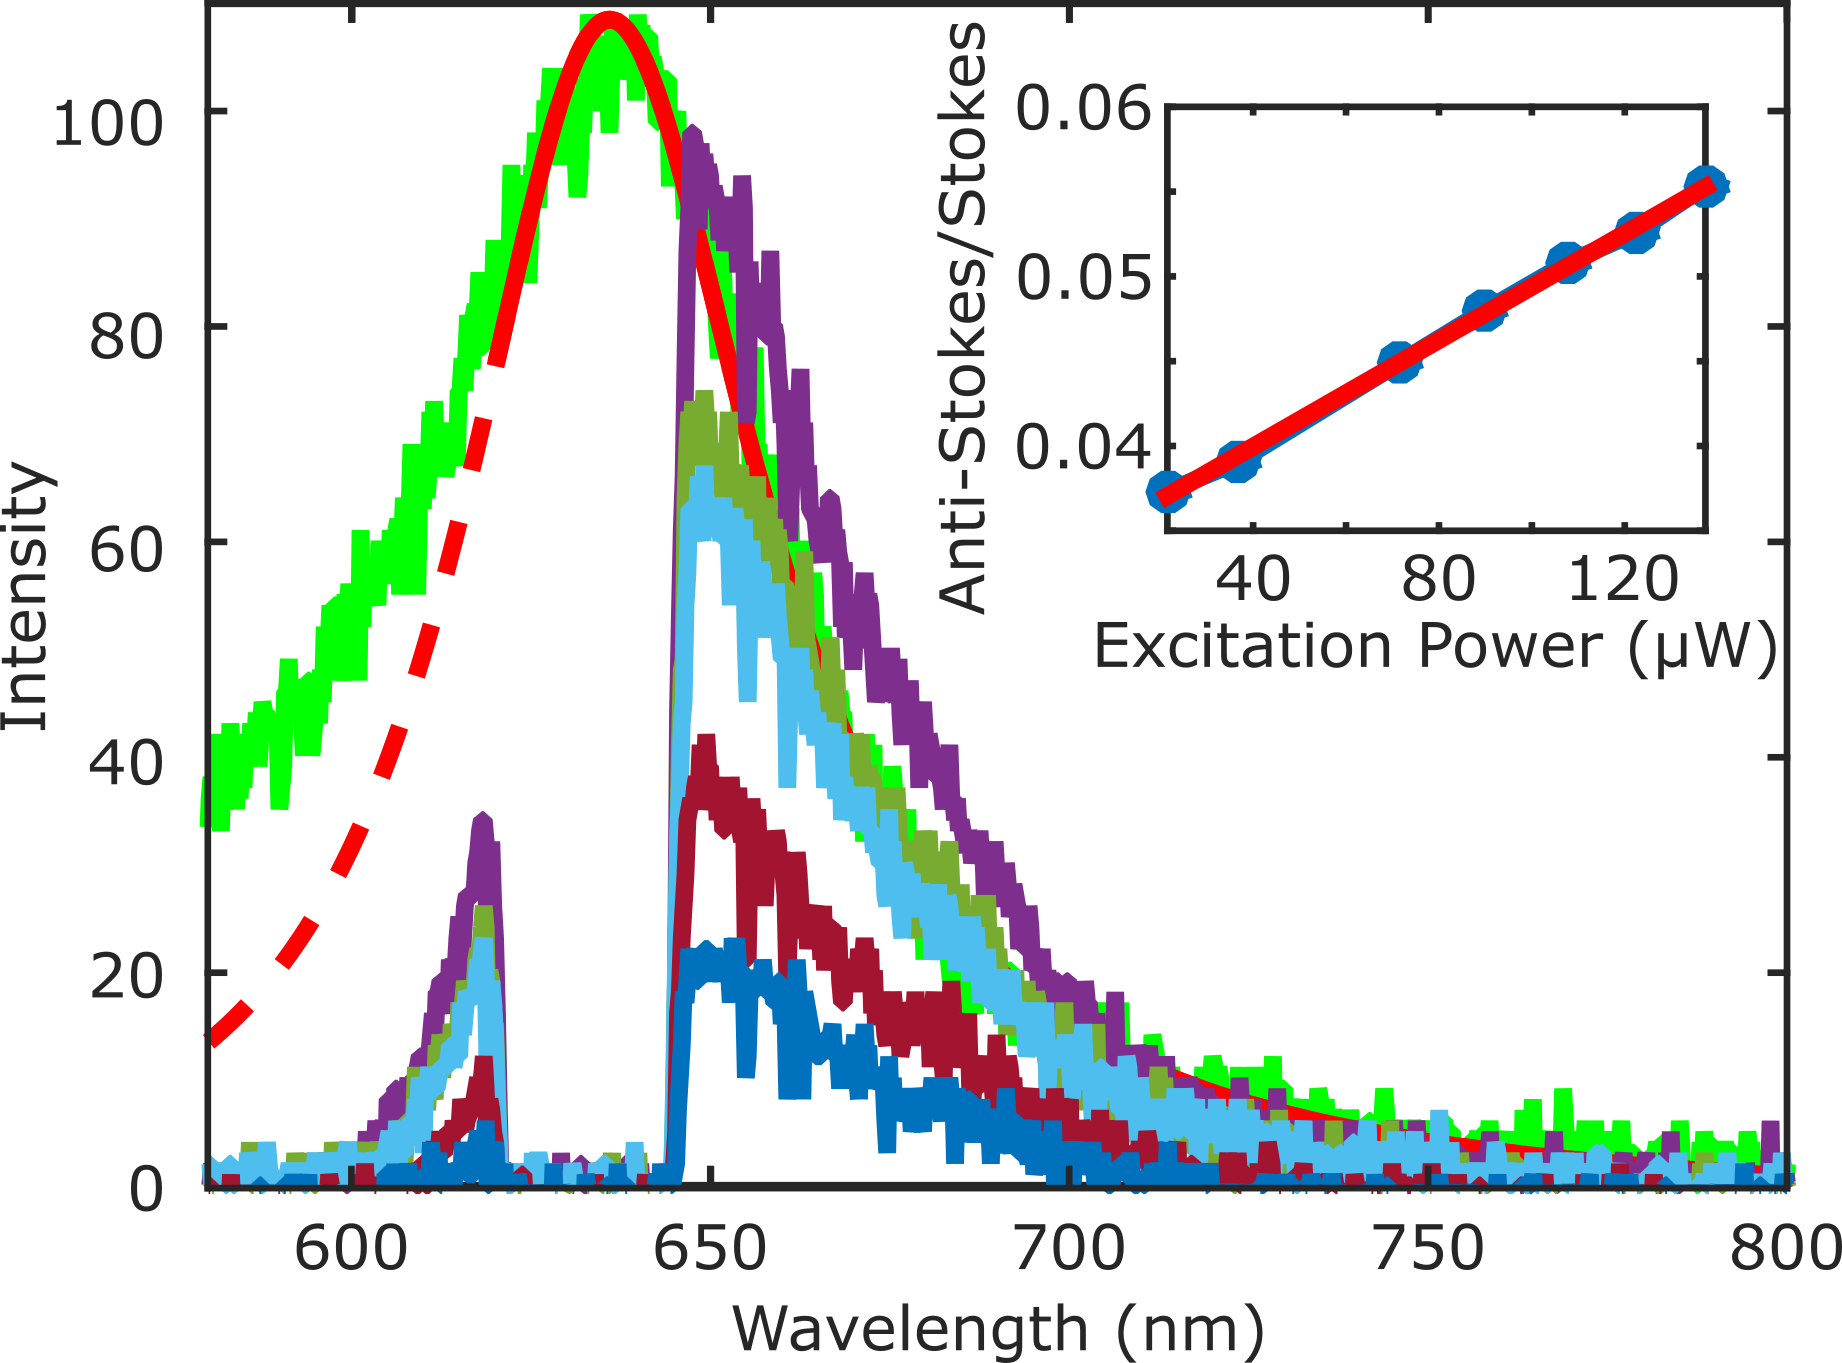
\includegraphics[width=78.4mm]{Figures/02_Several_Intensities/02_several_intensities.png}
\caption{\textbf{Luminescence emission spectra of a single gold nanorod.} The green curve is the
measured luminescence emission under $532\nm$ excitation with a Lorentzian fitting in red. The
dashed part is the region that was not considered for the fitting. The other
curves are the emission of the same particle under $633\nm$ irradiation at three 
different powers indicated in the legend. The inset shows the anti-Stokes-to-Stokes ratio as a function
of the excitation power, overlapped with a linear fit in red. The dip centered on the laser wavelength
is caused by the notch filter used to prevent the excitation laser from reaching the detectors.}
	\label{fig:spectra_intensity}
\end{figure}

The proposed model for the anti-Stokes emission requires to know the plasmon
spectrum ($\textrm{I}_{\textrm{SPR}}(\omega)$ in equation \ref{eqn:fitting}) of
the particle in order to fit the emission at shorter wavelengths and extract the
particle temperature. It has been shown that both scattering and luminescence
spectra roughly overlap over a broad range of wavelengths\cite{Yorulmaz2012}. Therefore
exciting gold nanorods with $532\nm$ allows us to record the longitudinal
plasmon spectra, as shown in the green solid curve of Figure \ref{fig:spectra_intensity}. The
peak was fitted by a single Lorentzian, shown in red in the Figure; the dashed
part of the curve is the spectral region that was not considered for the
fitting. It has to be recalled that the luminescence spectrum is not a perfect
Lorentzian since there is a broadband contribution to the luminescence arising
between the excitation wavelength and the plasmon peak\cite{Boyd1986}. This
appears as an asymmetry in the emission spectrum, particularly visible for
wavelengths smaller than $625\nm$. The results of this fitting will be employed
for the $I_\textrm{SPR}$ function defined in equation \ref{eqn:fitting}. 

The other curves in Fig. \ref{fig:spectra_intensity} show the luminescence emission of
the same nanorod while irradiating with a $633\nm$ laser at different powers,
ranging from $25\uW$ to $75\uW$ at the back aperture of the objective.  
%% should change to intensity or clearly mention the spot size
The vertical black line shows the wavelength of the laser. The Stokes part of the
spectrum at longer wavelengths than the excitation shows the same shape as the
plasmon emission observed under $532\nm$ excitation, apart from a normalization
factor. From the figure it can readily be seen that the shape of the anti-Stokes
emission, at shorter wavelengths than excitation, is exponential-like and
doesn't follow the Lorentzian shape of the Stokes emission. The dip between
Stokes and anti-Stokes is caused by the notch filter that prevents direct
excitation light from reaching the detectors. 

The inset of Figure \ref{fig:spectra_intensity} shows the anti-Stokes-to-Stokes ratio of
the integrated luminescence for different laser excitation intensities. It is
possible to see that even with a linear behavior, the anti-Stokes intensity
increases more rapidly with laser excitation power than the Stokes emission.
We already exploited this phenomenon to image gold nanorods in high-background
conditions\cite{Carattino2016a}. Moreover it shows that the anti-Stokes emission
depends on laser excitation power differently than its Stokes counterpart. For more 
information on the power dependence of both the anti-Stokes and Stokes luminescence, 
please refer to the Supplementary Information. 

\begin{figure}[tp] \centering
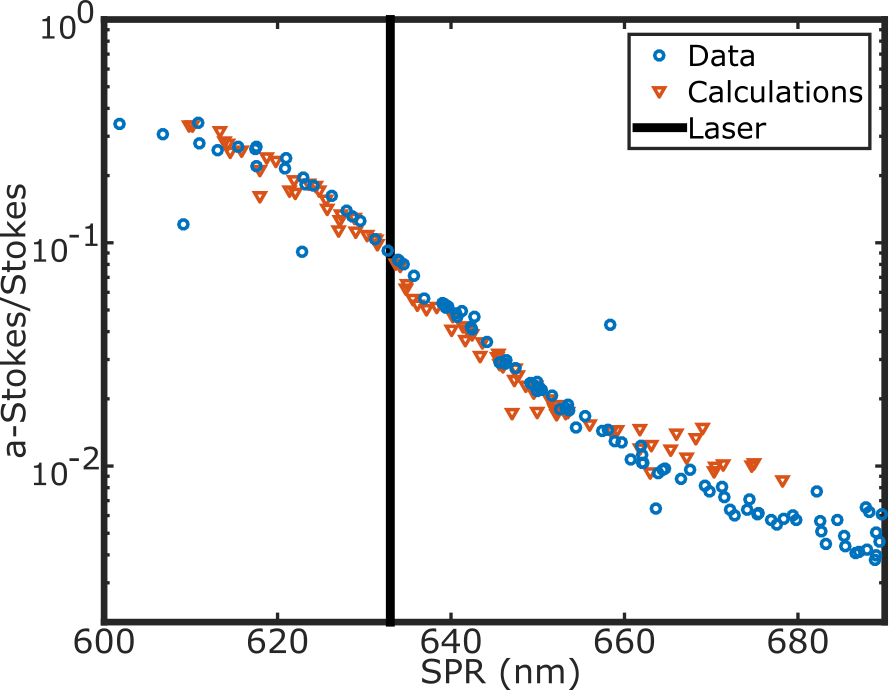
\includegraphics[width=75.5mm]{Figures/02_AS_vs_S_SPR/02_AS_vs_S_SPR.png}
\caption{\textbf{Characterization of anti-Stokes emission for different SPR.} 
Ratio of the anti-Stokes to Stokes emission under $633\nm$ excitation
as a function of the resonance wavelength of each particle.
The blue circles are experimental results, while the red triangles are the
results of the calculations with equation \ref{eqn:BE}. There is a very
good agreement between experiment and calculations. Particles with a resonance
to the blue of the laser (indicated by the vertical red line) have an increased anti-Stokes
emission.}
	\label{fig:ASS-ratio}
\end{figure}

To further characterize this phenomenon, we measured the emission for $90$
nanorods with different plasmon resonances under the same $633\nm$ excitation
and calculated the ratio of integrated anti-Stokes to Stokes emission.
Figure \ref{fig:ASS-ratio} shows the experimental results in blue circles, where
the horizontal axis of the figure is the surface plasmon resonance (SPR) of each
particle. The vertical red line marks the laser wavelength. The particles shown
in the plot had resonances between $600\nm$ and $690\nm$; the ones showing the
maximum ratio of anti-Stokes to Stokes are those with a resonance to the blue of
the laser. For these particles the longitudinal plasmon is enhancing preferably the
anti-Stokes emission. For particles with a resonance at the laser wavelength the
anti-Stokes and the Stokes emission have similar enhancement and show a ratio
close to $10\%$.

Figure \ref{fig:ASS-ratio} also shows the results of numerical calculations as the red
triangles. An excellent overlap between the measured and the calculated data can
be observed. The absorption cross section of several particles was calculated
with the ADDA package\cite{Yurkin2011}. Each calculated absorption spectrum was
fitted by a Lorentzian and used as $\textrm{I}_{\textrm{SPR}}(\omega)$ in eqn.
\ref{eqn:fitting}. Assuming a diffraction-limited laser spot and using the
\ref{eqn:fitting}. Assuming a diffraction-limited laser spot and using the
calculated absorption cross section allowed us to calculate the temperature of
the particle. This value was used in eqn. \ref{eqn:fitting} to compute the
anti-Stokes emission spectrum. The Stokes emission was set proportional to the
excitation power  with a shape given by the calculated absorption spectra. Since both
anti-Stokes and Stokes emissions are proportional to the excitation power, this
term cancels out when computing the ratio. The laser power therefore only enters
into the equation when calculating the temperature of the particles. It is
remarkable that the agreement between data and calculations was achieved
without free parameters, solely taking into account the transmission spectra of
the filters.

\begin{figure}[tp] \centering
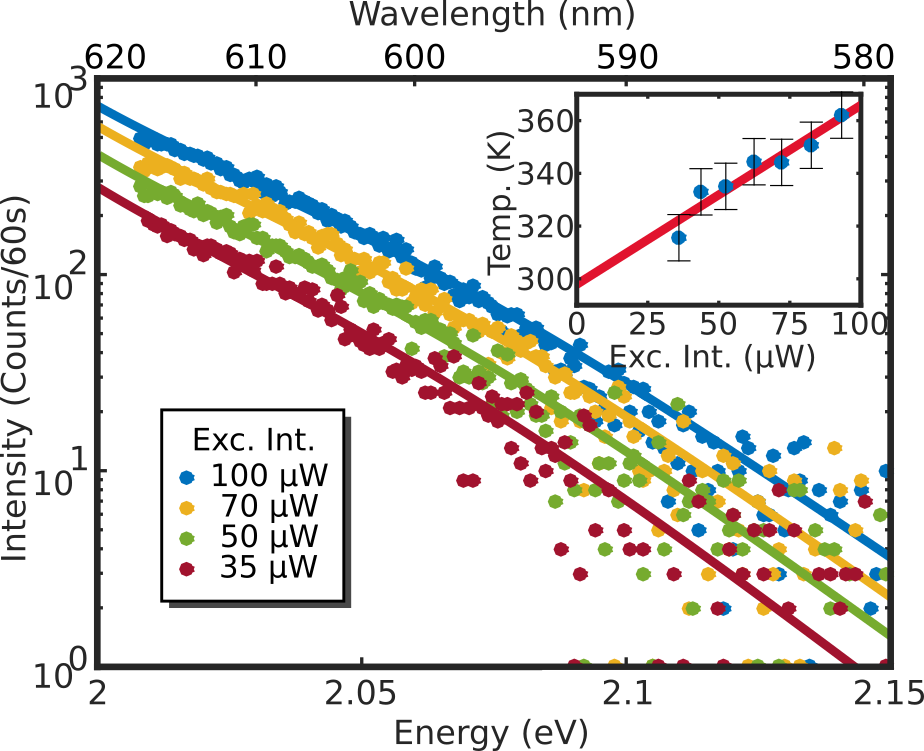
\includegraphics[width=78.4mm]{Figures/03_Fit_Of_AS/03_Log_Fit_AS.png}
\caption{\textbf{Anti-Stokes emission at different irradiation powers.} We used 
the model from equation \ref{eqn:fitting} to fit the experimental data. 
There is an excellent agreement between data and model. The inset shows the extracted
temperature at each power (blue dots) and a linear 
extrapolation of the data to $0\uW$ excitation power.
The value obtained for room temperature was $293\K$ while the measured value was
$296\K$.}
	\label{fig:AS_in_Log}
\end{figure}

Furthermore, by fitting the anti-Stokes part of the spectra shown in Figure
\ref{fig:spectra_intensity} with equation \ref{eqn:fitting} it is possible to extract
the temperature of the particle at each excitation power. Figure
\ref{fig:AS_in_Log} shows the results of this procedure. The spectra shown were
recorded at $4$ different excitation intensities while the full lines are the
fits; again, there is an excellent agreement between data and model. For every
anti-Stokes measurement we have also acquired the full plasmon spectrum while
exciting with a $532\nm$ laser before and after the temperature extraction.
The full plasmon spectrum is necessary to calculate the parameters of
$I_\textrm{SPR}(\omega)$ from equation \ref{eqn:fitting} and also to verify that the
particle did not reshape while being excited at resonance. 

The inset in Figure \ref{fig:AS_in_Log} shows the temperatures resulting from
the fits at different irradiation intensities (blue dots). It has to be noted
that the absolute temperatures of the particle at each excitation power were
calculated without any calibration. As expected, the temperature of the nanorod
is proportional to the excitation intensity, or equivalently to the absorbed
energy. Thus, this method provides an \textit{in situ} way to measure the
temperature reached by nanoparticles when they are excited with resonant
monochromatic light. Additionally, from these data sets it  is also possible to
calculate the temperature at $0\uW$ excitation power, i.e. room temperature, by
extrapolating the results with a linear fit. The value we obtained in this case
is $293\pm 6 \K$, while room temperature was $296\K$, a $2\%$ accuracy.

The accuracy of the obtained temperature depends to a great extent on the
plasmon resonance. The first step in the fitting procedure is the determination
of the term $I_\textrm{SPR}(\omega)$ in equation \ref{eqn:fitting}. This is achieved by
fitting a Lorentzian to the emission spectrum obtained while irradiating with a
$532\nm$ laser. In figure \ref{fig:spectra_intensity} it is possible to observe
that the emission spectrum is not perfectly Lorentzian and therefore the fitting
results will be sensitive to the portion of the spectrum selected. Depending on
the wavelength range selected, the parameters of the Lorentzian fit (its width
and peak position) can slightly change therefore giving rise to different
temperatures when fitting the anti-Stokes emission spectrum.

Equation \ref{eqn:fitting} shows that when the resonance is to the red
of the laser, the term $I_\textrm{SPR}(\omega)$ will slowly vary in the region where the
anti-Stokes emission is observed. Therefore small changes in the parameters of
the Lorentzian fit will have a small effect on the temperature extracted.
However, particles that are not in resonance with the excitation laser will
present a lower emission due to a smaller absorption cross section and to a
lower enhancement of the anti-Stokes emission (see for example figure
\ref{fig:ASS-ratio}). 
%A balance between the amount of collected light and the
%uncertainty produced by the correct determination of the plasmon resonance has
%to be reached depending on each application.
The error bar in figure
\ref{fig:AS_in_Log} and in the following figures is the result of the estimation
of the temperature uncertainty because of variations in the plasmon resonance
fit.

As expected from the model, the anti-Stokes emission should depend not only on
the particle's intrinsic properties but also on the temperature of the
surrounding medium\cite{Konrad2013}. In order to test this point, we changed the
temperature of the sample in a controlled manner and recorded the luminescence
emitted by a single nanorod.

For this set of experiments we employed an air objective ($60X$, NA $0.9$,
Olympus) to avoid the presence of a heat sink directly in contact with the
observed area. We employed higher laser powers to compensate for the lower
excitation efficiency. At each temperature several spectra were acquired at different
$633\nm$ excitation powers and also a spectrum of the plasmon before and after
each measurement in order to monitor any possible reshaping of the particles
during the experiment.

\begin{figure}[tp] \centering
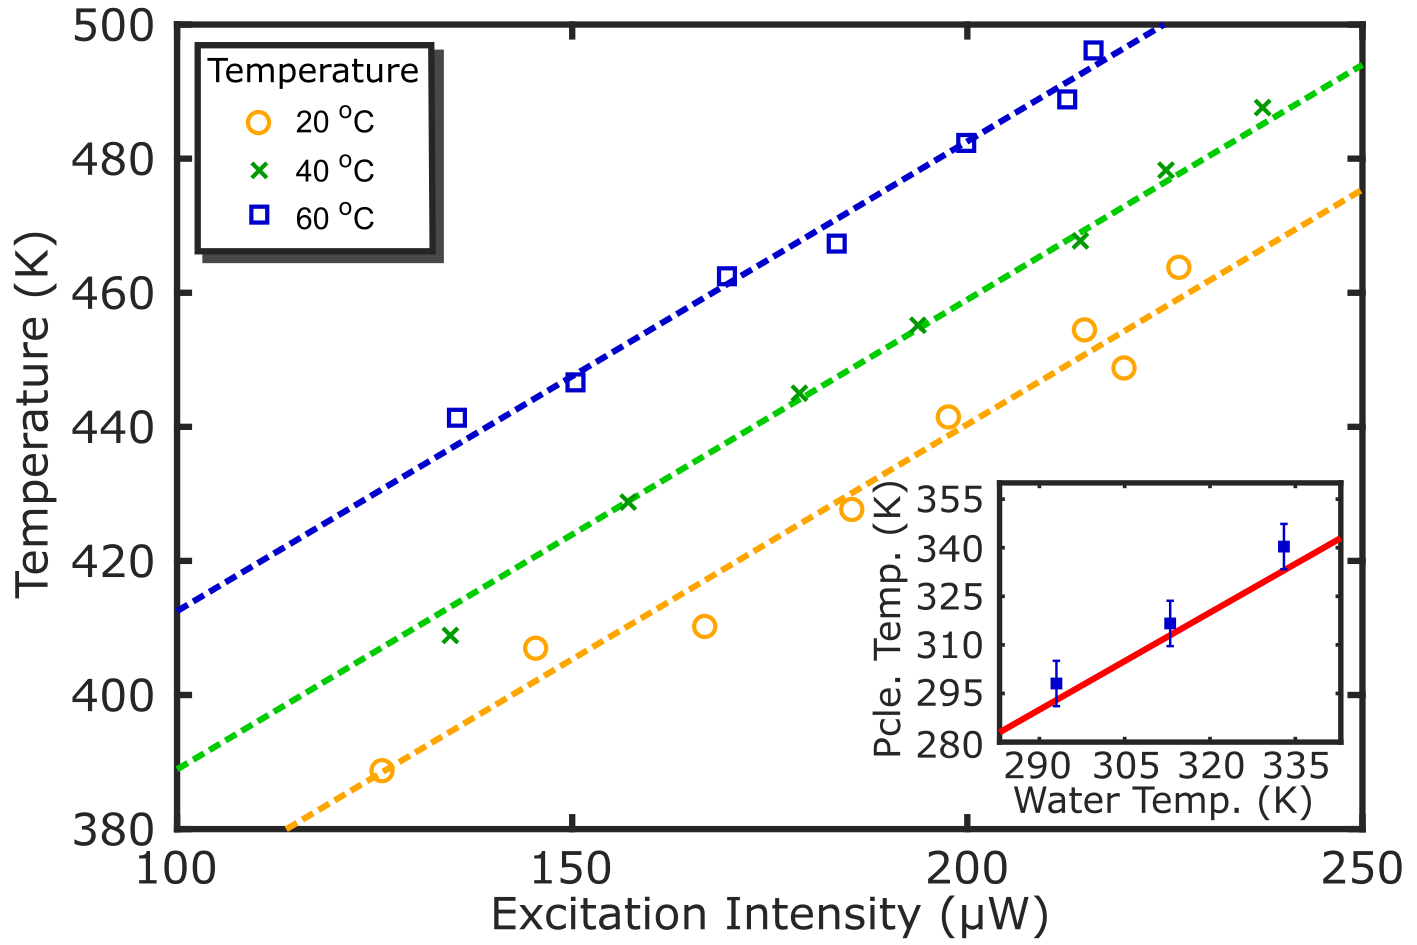
\includegraphics[width=88.4mm]{Figures/03_Fit_Of_AS/03_Log_Fit_AS_02.png}
\caption{\textbf{Calibration-free temperature measurement.}
Anti-stokes-luminescence extracted temperatures for an individual nanorod
at different excitation powers and at different sample temperatures. 
The dashed lines lines are fits with the same slope for the three temperatures. 
The circles in the inset plot show the local temperature of the sample obtained
by extrapolating temperature at zero excitation power as a function of the water temperature.
The red line represents the expected curve if both temperatures are identical (equal).}
	\label{fig:AS_temp}
\end{figure}

% this paragraph is not so clear to me since it looks there is a loop on the
% room temp determination

Figure \ref{fig:AS_temp} shows the extracted temperature of a particle at
varying excitation powers and at different water temperatures. The blue squares
are the results of the measurement at $20\degree$, while the green crosses are measured
at $40\degree$ and the yellow circles at $60\degree$. The full lines are the
calculated temperatures for a particle with plasmon overlapping the measured one
and assuming a diffraction-limited focus spot. For the dimensions of the
particle, the mean values from TEM images were used and the length was adjusted
to obtain the measured resonance. There is a remarkable agreement between the
calculation and the measured values. Moreover it is possible to extrapolate the
temperature at zero excitation power for each case as was explained earlier. The
results are shown in the inset of the figure for each temperature. The red line
with slope $1$ is a guide to the eye.

Figure \ref{fig:AS_temp} clearly shows that the extracted temperature varies
with the temperature of the surrounding medium. More strikingly the method does
not require any previous calibration nor adjustment. The values obtained with
the extrapolation to $0\uW$ excitation power were $298 \pm 7\K$, $316\pm 7\K$
and $340 \pm 6\K$ for water temperatures of $293\K$, $313\K$ and $333\K$
respectively. The calibration-free procedure would allow us to perform the same
measurements in any other setup and could act as a reference for calibration of
other nano thermometers.

%\section{Conclusions}

Being able to control and monitor temperature at the nanoscale is of utmost
importance in different fields ranging from photothermal therapy\cite{Huang2006}
to nano fabrication\cite{Fedoruk2013}. In this work we have shown a simple
procedure that allows us to measure the temperature of single gold nanorods
irradiated by a monochromatic continuous laser and without any previous
calibration. The level of accuracy of the temperature measurement depends on
several factors, but for nanorods it can be estimated to be better than $6\K$.

The model employed for describing the anti-Stokes emission takes into account
the plasmon, responsible for enhancing the emission, as well the electron-hole pairs
interaction with the thermal baths, where coupling to phonons is the dominant process.
It has been shown that the correct characterization of the plasmonic resonance is
fundamental for the proper extraction of temperature, specially in cases
where the resonance is to the blue of the excitation wavelength.

Particles with a resonance to the red of the excitation wavelength would be more
reliable in the temperature extraction procedure, but would also exhibit a lower
emission towards shorter wavelengths. The trade-off between both effects and
the possibility to fully characterize the plasmon resonance, will determine the
specific particles that are better suited for each application.

A possible improvement for this technique would be the use nanostructures with 
%of nanospheres.
%Since these particles do not reshape under higher excitation powers it is
%possible to compensate their lower cross section by increasing the irradiation
%intensity. However, their quantum yield is at least one order of magnitude
%smaller than that of rods, giving an overall lower photoluminescence intensity.
%Samples 
a narrow shape distribution such as gold
bipyramids\cite{Pelton2009}. Such structures would be ideal candidates for 
temperature extraction since they present negligible size dispersion and thus 
their plasmon can be measured in bulk or determined from theory, avoiding the need
of a second excitation source. This would reduce the main source of inaccuracies for the
method. 

The proposed method doesn't require any calibration, since the only free
parameter of the model is the absolute temperature of the nanoparticle under
study. Moreover the recording of the anti-Stokes spectrum is readily achievable
in any confocal microscope with a coupled spectrometer. A $6\K$ accuracy may
suffice for several applications; it is important to point out that this value
can be improved in different ways: by carefully selecting the particles that
show the most favorable plasmon resonance; by determining the plasmon resonance
through white-light scattering, avoiding the uncertainty in the fit; by
increasing the exposure times to increase the signal-to-noise ratio.

% %%%%%%%%%%%%%%%%%%%%%%%%%%%%%%%%%%%%%%%%%%%%%%%%%%%%%%%%%%%%%%%%%%%% % The
% "Acknowledgement" section can be given in all manuscript % classes.  This
% should be given within the "acknowledgement" % environment, which will make
% the correct section or running title.
% %%%%%%%%%%%%%%%%%%%%%%%%%%%%%%%%%%%%%%%%%%%%%%%%%%%%%%%%%%%%%%%%%%%%
\begin{acknowledgement}
This work is part of the research programme of the Foundation for Fundamental
Research on Matter (FOM), which is part of the Netherlands Organisation for
Scientific Research (NWO).
\end{acknowledgement}

%%%%%%%%%%%%%%%%%%%%%%%%%%%%%%%%%%%%%%%%%%%%%%%%%%%%%%%%%%%%%%%%%%%%%
%% The same is true for Supporting Information, which should use the
%% suppinfo environment.
%%%%%%%%%%%%%%%%%%%%%%%%%%%%%%%%%%%%%%%%%%%%%%%%%%%%%%%%%%%%%%%%%%%%%
\begin{suppinfo}
Scheme for the Au NR luminescenec mechanism.  Details concerning the experimental setup. 
Luminescence power dependence. Gold Nanorod temperature calculations.
\end{suppinfo}

%%%%%%%%%%%%%%%%%%%%%%%%%%%%%%%%%%%%%%%%%%%%%%%%%%%%%%%%%%%%%%%%%%%%%
%% The appropriate \bibliography command should be placed here.
%% Notice that the class file automatically sets \bibliographystyle
%% and also names the section correctly.
%%%%%%%%%%%%%%%%%%%%%%%%%%%%%%%%%%%%%%%%%%%%%%%%%%%%%%%%%%%%%%%%%%%%%

\bibliography{anti_stokes}
\end{document}
